\chapter{Tecnologie Utilizzate}
\label{cap:tecnologie}

In questo capitolo verranno descritte le tecnologie utilizzate nella realizzazione del progetto.

\section{HTML e CSS}
\subsection{HTML}
HTML, o HyperText Markup Language, è un liguaggio che permette di creare pagine web definendone la struttura, la quale verrà successivamente interpretata dal browser, principale strumento per la fruizione di pagine web.
Una pagina HTML è composta da elementi creati attraverso i cosiddetti tag html.
La struttura base di una pagina HTML è formata da 1 tag principale chiamato $<html>$  che conterrà altri 2 tag fondamentali, $<head>$  e $<body>$.
Nel tag $<head>$  si inseriranno informazioni non visibili nella pagina mostrata dal browser (fatta eccezione per il titolo della pagina), mentre nel $<body>$  andremo ad inserire tutto quello che l'utente andrà a vedere e con il quale potrà interagire.
Vediamo un esempio:
\begin{figure}[H]
    \centering
    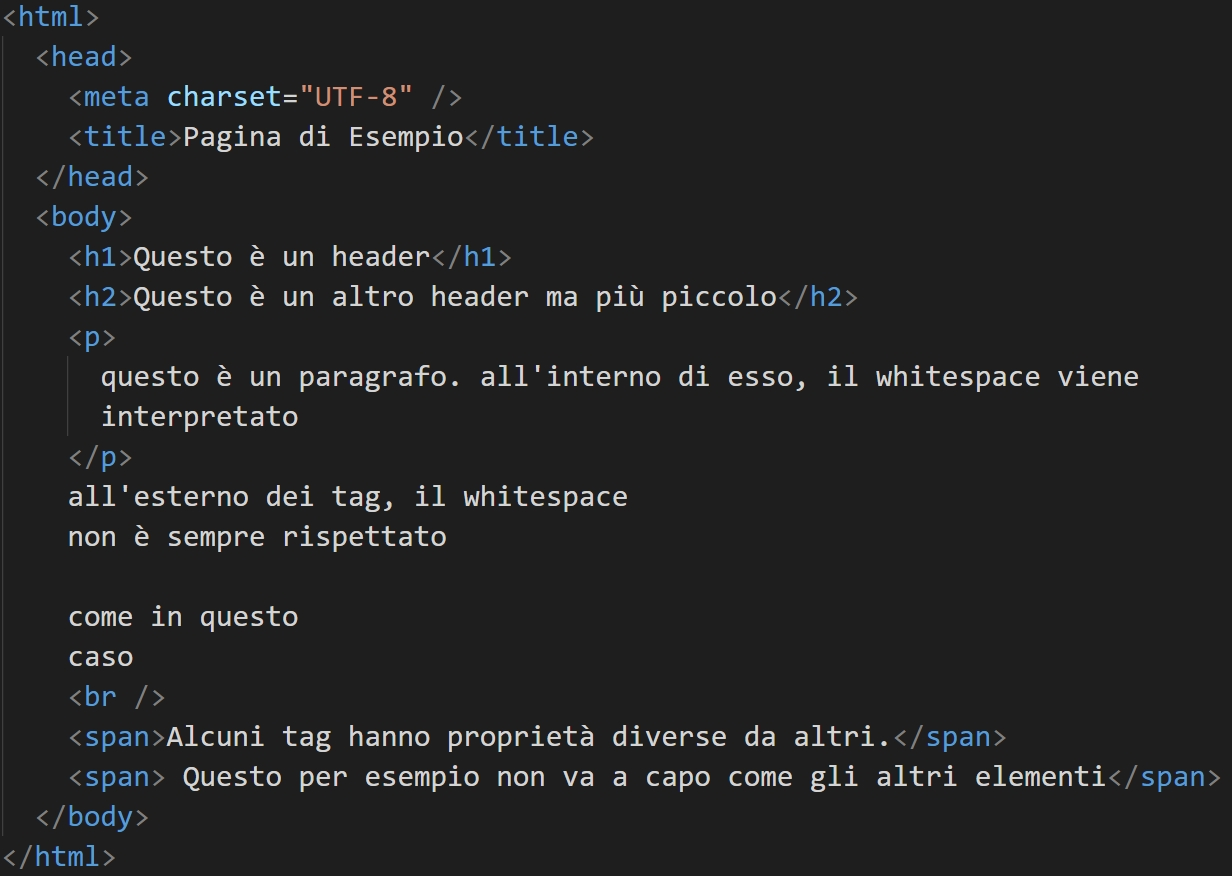
\includegraphics[scale=0.45]{images/html_code_example.jpg}
    \caption{Codice sorgente HTML}
    \label{fig:codice_html}
\end{figure}
\begin{figure}[H]
    \centering
    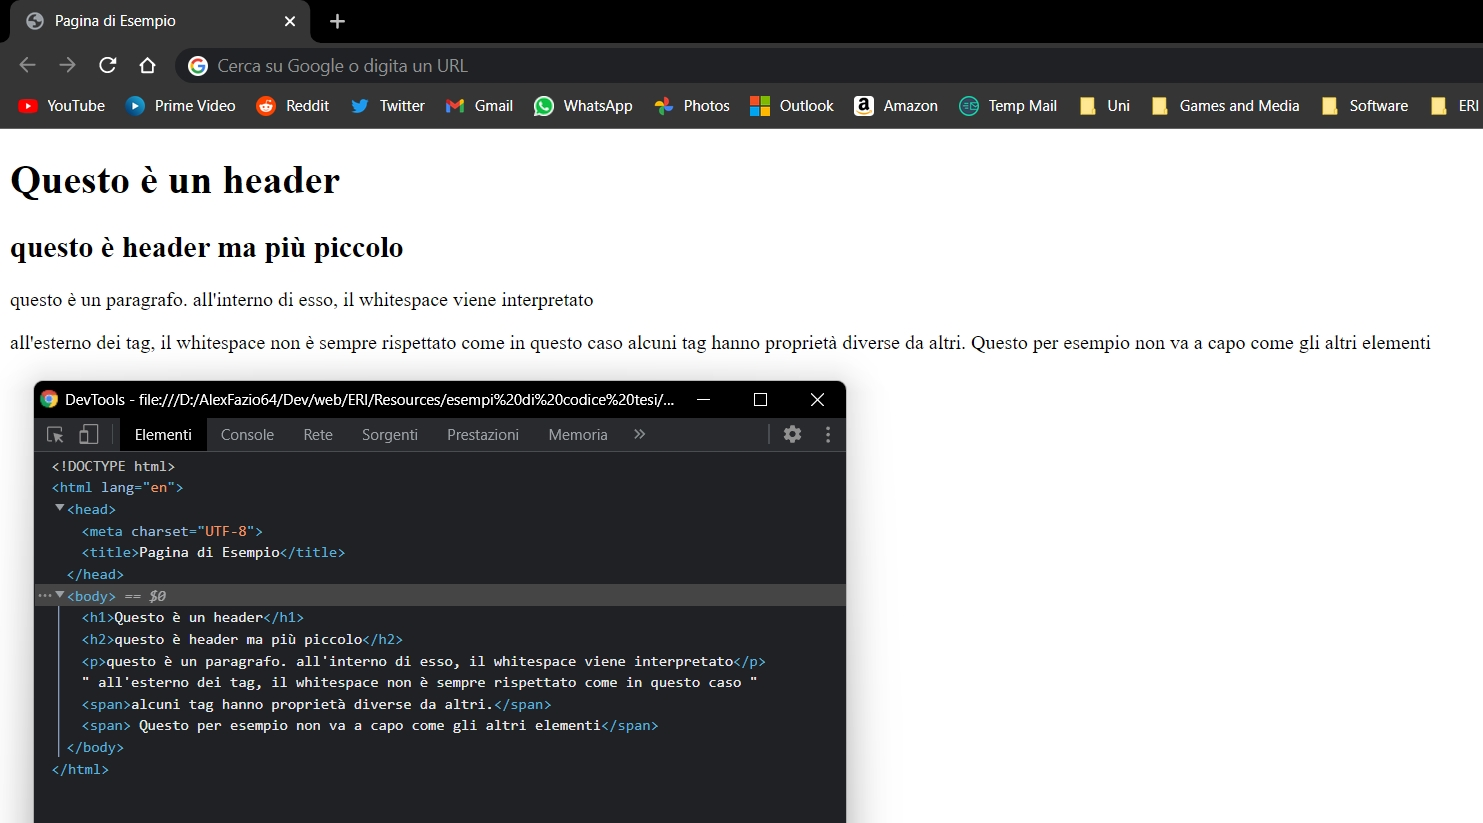
\includegraphics[scale=0.4]{images/browser_interpretation.jpg}
    \caption{Pagina web interpretata dal browser}
    \label{fig:pagina_nel_browser}
\end{figure}
HTML rende possibile la creazione di una pagina interattiva basilare, ma grazie a linguaggi di supporto quali CSS e Javascript è possibile stilizzare il contenuto ed eventualmente cambiare il comportamento standard degli elementi.
\subsection{CSS}
CSS, acronimo di Cascading StyleSheets permette di personalizzare il modo in cui il browser mostra il contenuto della pagina HTML al quale viene applicato.
Vengono introdotti nuovi concetti in modo da applicare lo stile selettivamente.
Concetti come regole, proprietà e selettori rendono possibile specificare uno stile diverso da quello di default del browser. Vediamo un esempio:
\begin{verbatim}
    p {
        color: red;
        font-size: 24pt;
        color: green;
    }
\end{verbatim}
In questo spezzone di codice è rappresentata una regola.
\begin{itemize}
    \item p è un selettore che identifica ogni tag $<p>$  indistintamente
    \item color e font-size delle proprietà
    \item red, 24pt e green sono valori
\end{itemize}
Questa regola renderà ogni paragrafo di colore verde e con font impostato a 24pt, questo poichè le regole e le proprietà vengono applicate a cascata (Cascading appunto).
Dato che color viene ridefinita più volte, l'ultima definizione avrà la priorità.

\section{Javascript e Typescript}
\subsection{Javascript}
Javascript è un linguaggio di scripting utilizzato principalmente per lo sviluppo di applicazioni web.
Grazie ad esso è possibile rendere dinamiche le pagine web reagendo alle azioni dell'utente.
Rende possibile modificare il comportamento standard degli elementi interattivi nelle pagine.
E' un linguaggio basato su multipli paradigmi, interpretato, debolmente tipizzato.
Tutti i browser moderni permettono alle pagine web di eseguire codice Javascript in un ambiente isolato, ovvero, ogni pagina può eseguire il proprio codice ma senza accedere al codice di altre pagine.
Esistono vari modi di includere codice Javascript all'interno di pagine html, ma il più comune è quello di importare il file .js all'interno di un tag $<script>$.
\subsection{Typescript}
Typescript è una versione tipizzata di Javascript, come suggerisce il nome.
Segue tutte le regole dello standard Javascript, ma rende più semplice l'implementazione e il debugging del codice da parte dello sviluppatore grazie a strumenti integrati negli ambienti di sviluppo.
I browser però non riescono ad interpretare codice scritto in Typescript dato che ha una notazione diversa, c'è quindi bisogno di tradurre tale prodotto in codice Javascript valido, e questo passo è fortunatamente automatizzato grazie a software appositi.

\section{Python}
Python è un liguaggio ad alto livello, interpretato e multiparadigma.
E' un linguaggio multiuso con il quale si possono implementare applicazioni di ogni tipo.
E' caratterizzato dalla somiglianza al linguaggio naturale e dalla sua notazione minimale che enfatizza la semplicità di implementazione.
E' stato scelto il suo utilizzo nel progetto proprio per la sua immediatezza e semplicità.

\section{Firebase}
Firebase è un servizio di Backend-as-a-Service (BaaS) offerto da Google.
Fornisce librerie in diversi linguaggi per intergrare tale servizio nelle applicazioni.
Tra i principali servizi offerti e utilizzati nel progetto abbiamo un Database Realtime e il servizio di Autenticazione.
Tali servizi sono già implementati e testati da esperti del settore in modo tale da semplificare il lavoro agli sviluppatori, i quali potranno usufruirne gratuitamente o a pagamento, ovviamente con ulteriori benefici e servizi avanzati.
Questo lavoro di tesi utilizza il piano gratuito offerto da Firebase poichè non si è necessitato di ulteriori funzionalità e dove necessario si è utilizzata una alternativa gratuita sfruttando un altri servizi.

\subsection{Realtime Database}
Il Realtime Database offerto da Firebase è un database JSON (JavaScript Object Notation) ottimizzato in modo tale da avere un bassissima latenza.
E' stato scelto tale database poichè i dati necessari al funzionamento della applicazione sono rappresentabili facilmente come JSON, e la bassa latenza aiuta con la reattività dell'assistente virtuale data la sua natura conversazionale.

\section{Svelte}
Svelte è un compilatore in grado di generare applicazioni web collegando la logica alla grafica attraverso una sintassi simile ad HTML e Javascript.
Permette allo sviluppatore di scrivere meno codice rispetto all'approccio tradizionale, e lo fa estendendo la sintassi standard in modo da rimanere familiare, ma introducendo concetti che facilitano lo sviluppo.
Svelte è basato su un approccio a componenti riutilizzabili. La struttura tipica di un componente è la seguente:

\begin{itemize}
    \item un tag $<script>$ locale al componente, all'interno del quale possiamo specificare la logica
    \item un tag $<style>$ dove possiamo personalizzare il modo in cui esso viene renderizzato dal browser
    \item una sezione in cui possiamo includere i tag standard di HTML
\end{itemize}

Il principale vantaggio di utilizzare Svelte è, come già accennato, il binding tra logica e grafica, e la semplicità con il quale viene realizzato.
\subsection{Frameworks}
Tradizionalmente per cambiare il comportamento di un bottone sono necessari 3 file diversi, un file .html dove definiamo la struttura della pagina, un file .js nel quale andiamo a selezionare il bottone in maniera molto verbosa, e un file .css dove personalizziamo lo stile di tale bottone.
Con Svelte basta un solo file .svelte che verrà successivamente compilato in diversi file a seconda delle funzionalità implementate.
Esistono altri strumenti, anche chiamati framework, simili a Svelte che permettono di sviluppare webapp facilitando il lavoro dello sviluppatore, per esempio:

\begin{itemize}
    \item React
    \item Vue
    \item Angular
    \item molti, molti altri\dots
\end{itemize}

Si è scelto di utilizzare Svelte per la realizzazione dell'interfaccia, per la quantità minimale di codice boilerplate necessaria rispetto ad altri framework, la leggibilità, le alte prestazioni e il supporto nativo a Typescript.

\begin{figure}[H]
    \centering
    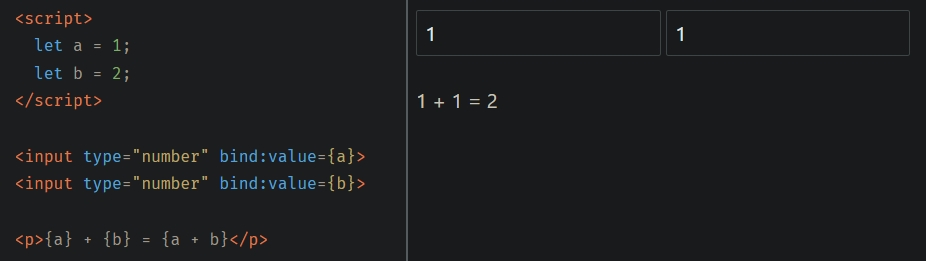
\includegraphics[scale=0.7]{images/svelte_example.jpg}
    \caption{Esempio di applicazione Svelte che sincronizza i valori di 2 $<input>$ sommandoli e stampandoli in un paragrafo }
    \label{fig:svelte_example}
\end{figure}
\begin{figure}[H]
    \centering
    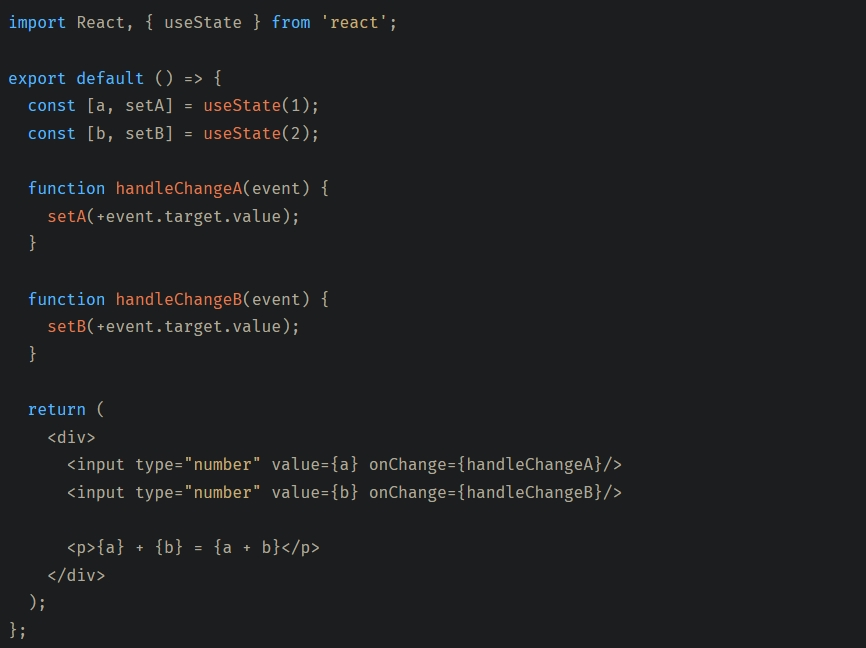
\includegraphics[scale=0.7]{images/react_example.jpg}
    \caption{La stessa applicazione ma scritta in React}
    \label{fig:react_example}
\end{figure}
\begin{figure}[H]
    \centering
    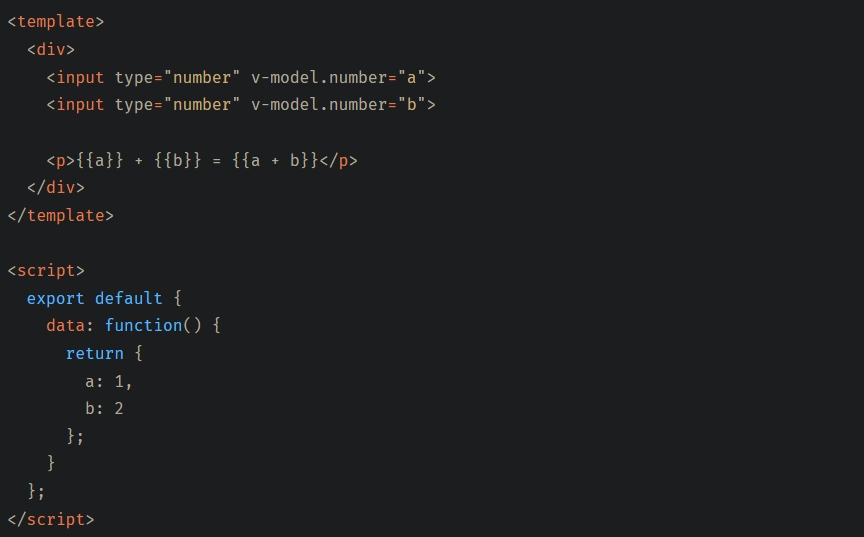
\includegraphics[scale=0.7]{images/vue_example.jpg}
    \caption{La stessa applicazione ma scritta in Vue}
    \label{fig:vue_example}
\end{figure}
\textbf{N.B:} esempi di codice presi da svelte.dev

\section{Sveltekit}
Sveltekit è un framework che include Svelte ed aggiunge ulteriori funzionalità com.



Sveltekit è un framework basato su Svelte che permette di creare applicazioni web fornendo un’esperienza di sviluppo più comoda e rapida. Diversamente dalle altre applicazioni basate su server side rendering, SvelteKit rende l’esperienza più rapida e fluida. \'E basato su Snowpack, un tool che velocizza il processo di sviluppo, compilando i file una singola volta e, successivamente, ricompilandoli solamente in caso di cambiamenti all'interno del codice. Il punto di forza di Sveltekit è la possibilità di avere un routing delle pagine basato sul file-system; ciò significa che la struttura dell’applicazione è basata sulla struttura del codice. Quindi, come per React, non c’è bisogno di utilizzare un router esterno per la propria applicazione web, come ad esempio Redux. Le funzionalità di Sveltekit sono numerose e la principali utilizzate in questo progetto sono state il \textit{server-side rendering} e il \textit{routing dinamico}.

\section{NodeJS e NPM}
\subsection{NodeJS}
NodeJS (o più semplicemente, Node) è una implementazione di ambiente runtime per Javascript basato su V8, l'ambiente runtime presente sul browser Chrome.
Permette di eseguire codice Javascript senza necessità di un browser.
Questo permette a Javascript di diventare un linguaggio multifunzione con la possibilità di realizzare applicazioni non per forza legate all'ambiente web.
Node aggiunge fornisce altre funzionalità, come l'interazione con il sistema operativo sul quale viene eseguito, il che lo rende il candidato perfetto per questo tipo di progetto.

\subsection{Node Package Manager}
NPM è un gestore di pacchetti per Javascript ed è il gestore di pacchetti predefinito su Node.
Un pacchetto software, in generale, è un insieme di programmi distribuiti congiuntamente che risolvono un problema specifico, in questo caso, un insieme di file Javascript correlati tra loro.
Con NPM è possibile integrare pacchetti realizzati da altri utenti nel proprio progetto, semplificando l'implementazione di funzionalità necessarie.
Un esempio di pacchetto utilizzato all'interno di questo progetto è appunto Firebase.

\section{Express}
Express JS

\section{Heroku}
Heroku

\section{Actions on Google}
Actions on Google
\subsection{Google Assistant}
Google Assistant
\subsection{Actions Console}
Actions Console